%!TEX program = xelatex
%%%%%%%%%%%%%%%%%%%%%%%这是导言部分的开始%%%%%%%%

%========= 导言部分声明文档的类型=================
\documentclass{article}

%=========导言部分可可以加载宏包=================
\usepackage{amsmath}                % 数学公式排版宏包
\usepackage{amssymb}                % 数学符号命令宏包
\usepackage{amsthm}                 % 数学定理宏包
\usepackage[UTF8]{ctex}             % 中文输入宏包
\usepackage[a4paper]{geometry}      % 页面设置宏包
\usepackage{setspace}               % 行间距宏包
\usepackage{graphicx}               % 图片宏包
\usepackage{listings}               % 代码宏包
\usepackage{color}					% 颜色宏包
\usepackage{xcolor}                 % 颜色处理宏包
\usepackage{float}                  % 浮动对象式样宏包
\usepackage{fontspec}
\usepackage{enumerate}				% 列举编号包

%=========页面设置==============================
\geometry{left=1cm,right=1cm,top=1cm,bottom=2cm}
\onehalfspacing
\setlength\parindent{0em}

%=========代码格式设置============================
\definecolor{dkgreen}{rgb}{0,0.6,0}
\definecolor{gray}{rgb}{0.5,0.5,0.5}
\definecolor{mauve}{rgb}{0.58,0,0.82}
% \setmonofont{Consolas}
\lstset{
	numbers = left, 	
	numberstyle = \color{gray}, 
	keywordstyle = \color{blue},
	commentstyle = \color{dkgreen}, 
	stringstyle = \color{mauve},
	basicstyle = \ttfamily,
	breaklines = true,
	frame = shadowbox, % 阴影效果
	rulesepcolor = \color{ red!20!green!20!blue!20} ,
	escapeinside = ``, % 英文分号中可写入中文
	xleftmargin = 2em,xrightmargin=2em, aboveskip=1em,
	framexleftmargin = 2em
} 

%=========导言部分可以定义标题信息===============
\title{组会报告}
\author{徐益}
\date{\today}
%%%%%%%%%%%%%%%%%%%%%%%这是导言部分的结束%%%%%%%%%

%%%%%%%%%%%%%%%%%%%%%%%这是正文部分的开始%%%%%%%%%
\begin{document}

%=========生成标题================================
\maketitle

%=========开始正文的输入==========================

%===========第一节=================
\section{工作内容} 
1. 完成服务器环境配置;

2. 学习线程绑定CPU;

3. 编写多线程编码调制模块。

%===========第二节=================
\section{服务器环境配置信息}
\lstset{language=C++}
\begin{lstlisting}
ubuntu: 16.04
gcc:    5.4.0
icc:    18.0.2
boost:  1.58.0
DPDK:   18.05.1
\end{lstlisting}

%===========第三节=================
\section{线程绑定CPU}
\subsection{CPU亲和度(affinity)}
\subsubsection{基本概念}
亲和度(affinity)是一种调度属性(scheduler property), 它可以将一个进程“绑定” 
到一个或一组CPU上。在SMP(Symmetric Multi-Processing对称多处理)架构下,
Linux调度器(scheduler)会根据CPU affinity的设置让指定的进程运行在“绑定”的CPU上,
而不会在别的CPU上运行。
\subsubsection{表示方法}
CPU affinity 使用位掩码(bitmask)表示, 每一位都表示一个CPU, 置1表示“绑定”。
最低位表示第一个逻辑CPU, 最高位表示最后一个逻辑CPU。

\subsection{核心函数}
\lstset{language=C++}
\begin{lstlisting}
NAME
	   pthread_setaffinity_np, pthread_getaffinity_np
	    - set/get CPU affinity of a thread

SYNOPSIS
       #define _GNU_SOURCE
       #include <pthread.h>
       int pthread_setaffinity_np(pthread_t thread, size_t cpusetsize,
                                  const cpu_set_t *cpuset);
       int pthread_getaffinity_np(pthread_t thread, size_t cpusetsize,
                                  cpu_set_t *cpuset);

       Compile and link with -pthread.
\end{lstlisting}

\subsection{测试结果}
\begin{figure}[H]
	\centering
	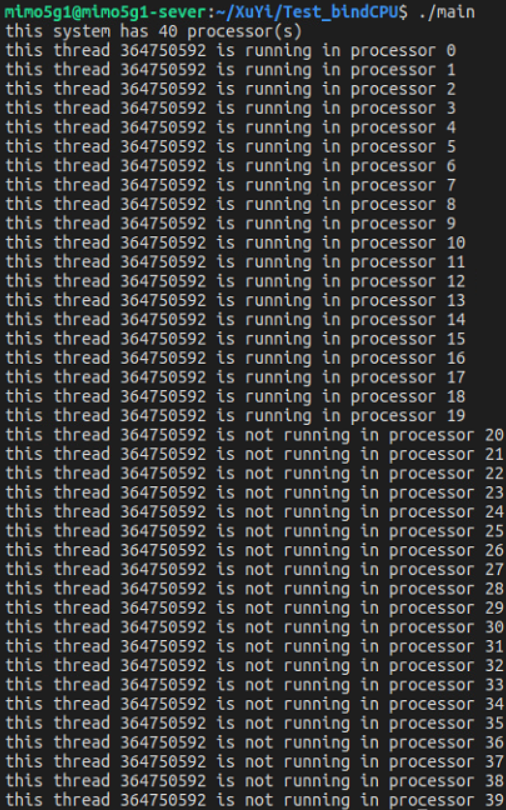
\includegraphics[width = .6\textwidth]{testCPU.png}
	\caption{测试结果}
\end{figure}

%===========第四节=================
\section{编写多线程编码调制模块}
\subsection{多线程结构}
\begin{figure}[H]
	\centering
	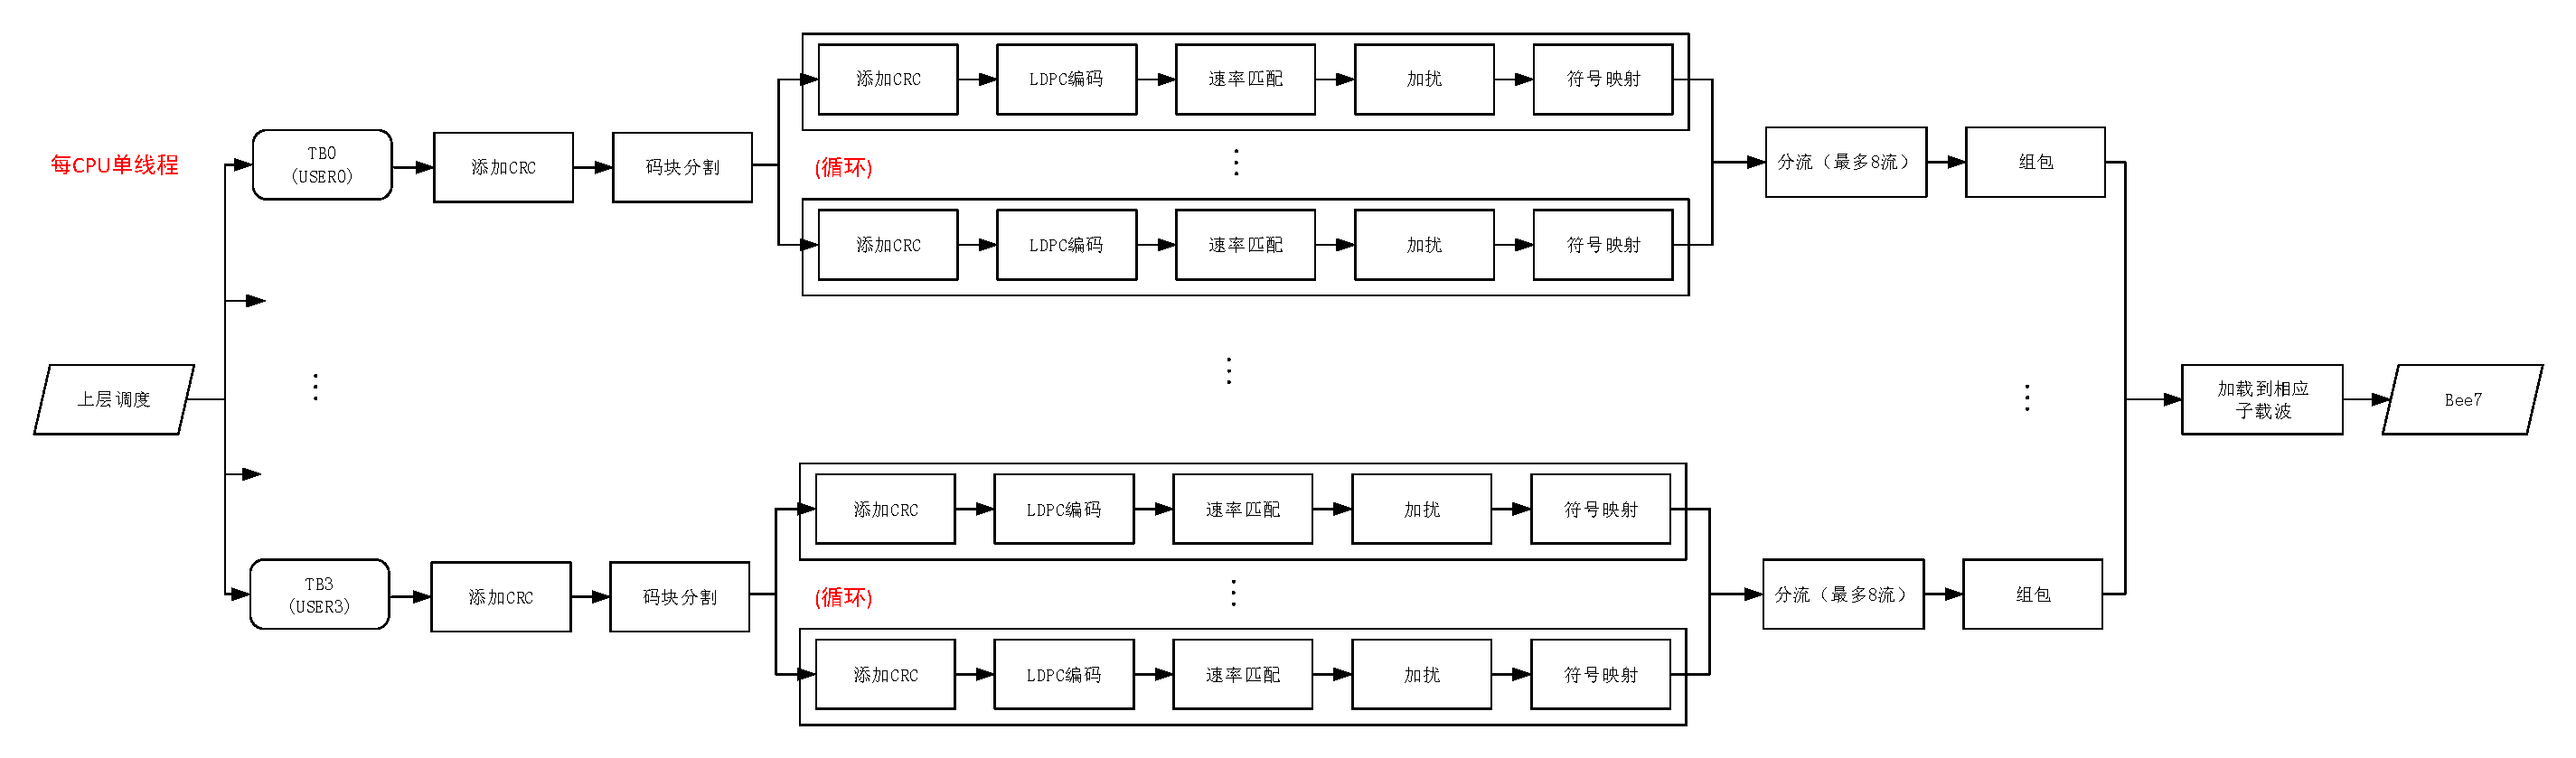
\includegraphics[width = \textwidth]{txstru.pdf}
	\caption{Tx结构}
\end{figure}
\begin{figure}[H]
	\centering
	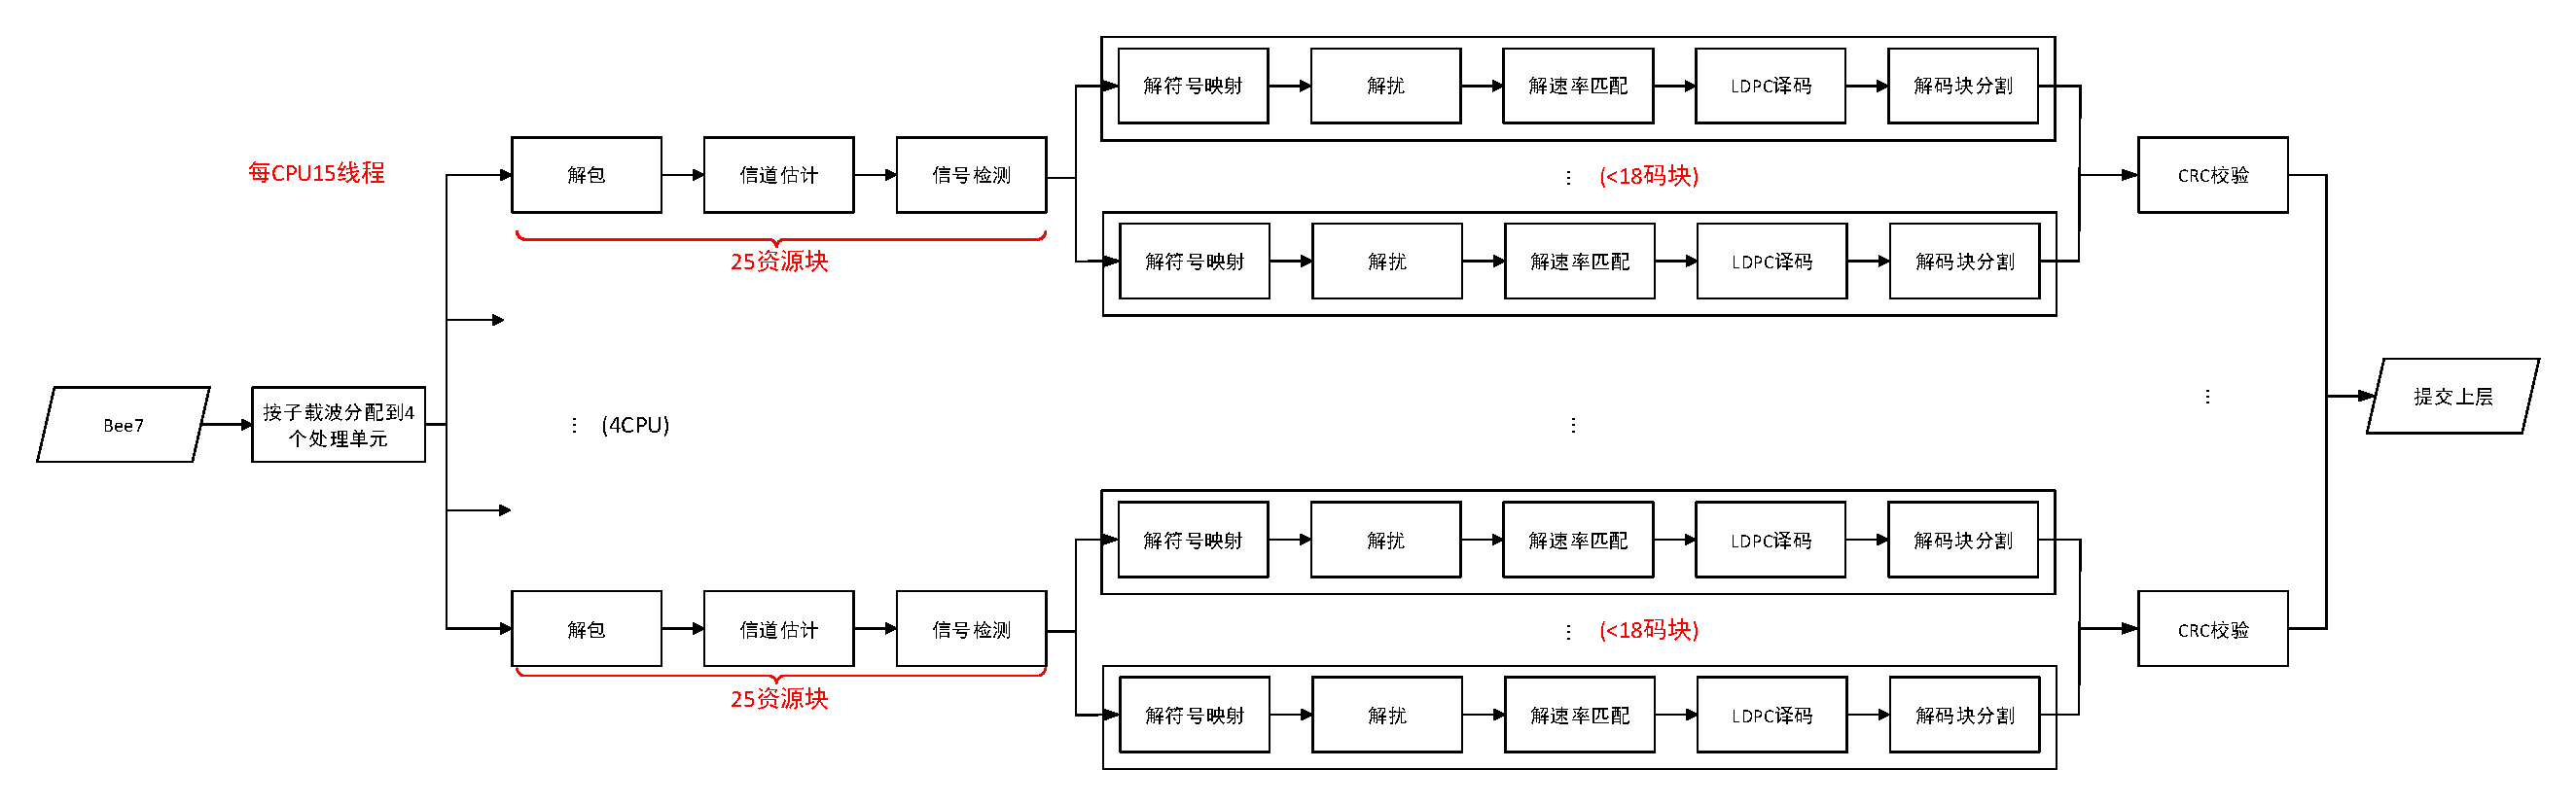
\includegraphics[width = \textwidth]{rxstru.pdf}
	\caption{Rx结构}
\end{figure}
\subsection{修改点}
1. 信号量传递由全局变量改为线程传参;\\
2. 轮巡式调度改为信号量调度; \\
3. 尝试简化线程阶段。

%===========第五节=================
% \section{有PRACH情况下的资源分配问题}
% \begin{figure}[H]
% 	\centering
% 	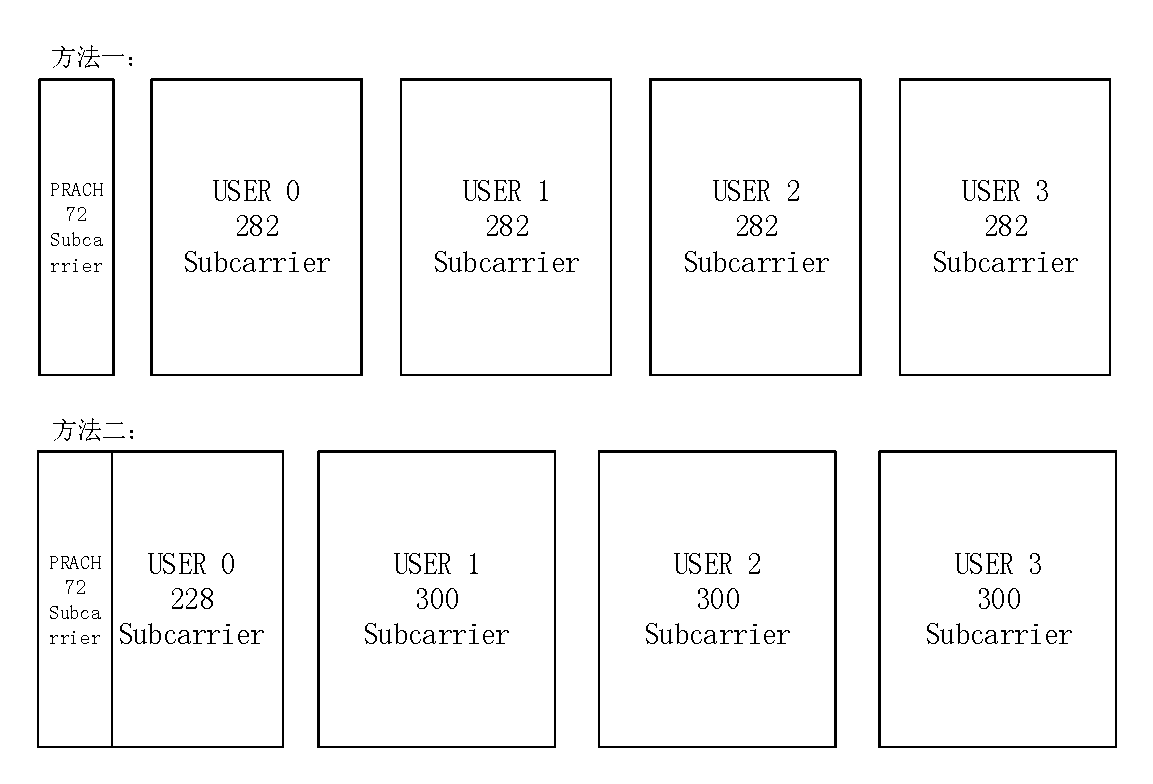
\includegraphics[width = \textwidth]{ques.pdf}
% 	\caption{两种方案}
% \end{figure}

%===========下周计划=================
% \section{下阶段计划}
% 1. 完善单线程系统(修复Bug)

\end{document}
%%%%%%%%%%%%%%%%%%%%%%%这是正文部分的结束%%%%%%%%%%%%